\documentclass{article}

\usepackage{mathtools}
\usepackage[margin=0.5in]{geometry}
\usepackage{graphicx}
\usepackage{caption}
\usepackage{subcaption}
\usepackage{hyperref}
\usepackage{booktabs}
\usepackage{float}
\usepackage{multirow}

\setlength{\parindent}{0pt}
\graphicspath{ {./experiment/data/} }

\title{Edge Detection Evaluation of HEp-2 Cells in Fluorescent Images}
\author{Ossama Edbali - ID: 1466610}

\begin{document}
	
	\maketitle	
	
	\section{Aim}
	
	This study aims to analyse the results and efficacy of several edge detection algorithms
	on HEp-2 cells.
	
	The edge detection/segmentation algorithms used are: Otsu, Sobel, Roberts, Canny,
	Canny using anisotropic diffusion,
	Laplacian of Gaussian, Difference of Gaussians, dilate-erode method and localised
	histogram edge detection (the last one is my development).
	
	The evaluation of each method is carried by ROC curves, sensitivity-specificity variation graph and correspondence analysis.
	
	\textbf{All the Matlab code and full data can be found here: \url{https://github.com/UoBCS/hep2-edge-detection}.}
	
	\section{Method}

	Given the three images (9343 AM, 10905 JL and 43590 AM) it can be seen that they
	are the outcome of different fluorescence patterns on the HEp-2 cells.
	First of all the experiments where conducted using three main scripts:
	\texttt{x9343AMtask}, \texttt{x10905JLtask} and \texttt{x43590AMtask}.
	
	Each script loads the relative image and true edge image (1). Then converts the original image to a grey-scale image using the \texttt{rgb2gray} Matlab function (2).
	Finally, it performs all the edge detection algorithms described above (delegating
		to the class \texttt{EdgeDetection.m}) (3).
	
	A pre-analysis (qualitative) of the input has been carried out using the
	background approximation image as a surface to see where illumination varies (using \verb|show_background| function).
	It can be seen that the various input images use different fluorescence patterns on
	the HEp-2 cells.	
	
	For all edge detectors there is a method inside the \texttt{EdgeDetection} class
	as well as methods for generating the ROC space and specificity and sensitivity
	in function of some parameters (e.g. threshold, sigma, number of iterations).
	
	For Roberts and Sobel a function \verb|detect_edges(img, filterX, filterY)| was developed which convolves \verb|img| with the two filters and uses
	\verb|magnitude| to produce the final result (before thresholding).
	
	In regards to LoG, Gaussian smoothing was performed using \verb|gaussian_smoothing(image, sigma)|. Then convolve the smoothed image with the laplacian
	operator and finally find the zero crossings: \verb|edge(res, 'zerocross')|.
	
	\subsection*{Otsu's method}
	One of the algorithms used in this study is the Otsu's algorithm.
	The aim is to find the threshold value where the sum of foreground and background spreads is at its minimum. First of all I calculate the weighted mean and variance
	for both the background and foreground ($\mu_b$, $\sigma_b^2$ and
	$\mu_f$, $\sigma_f^2$). Then I compute the \textbf{within-class variance} (two variances multiplied by their associated weights): $\sigma_W^2 = W_b \sigma_b^2+W_f \sigma_f^2$. I do the same calculation for candidate thresholds and the one that has the lowest within-class variance will be chosen. This algorithm is implemented in the Matlab's
	\verb|graythresh|. This will produce a binary image which edges' can be detected
	easily by any of the edge detectors (Sobel in the experiment).
	
	\subsection*{Dilate-erode method}	
	
	The dilate-erode method is a 4-step algorithm that uses a combination of  morphological operators before using Sobel edge detector. The reason why this method
	has been used is that when Sobel (or Roberts) is performed on the grey-scale image, there are some lines of high contrast surrounding
	the actual edge (like noise). The gaps between these small lines and the actual edge
	can be filled using a \textbf{dilate morphological operator} (or non-linear neighbourhood
	operator) with a structuring element (from the \verb|strel| function). Then
	\verb|imfill| has been used to fill the holes inside the cell.
	The next step is to reduce to get the cell back to its state before dilation using
	the \textbf{erosion} operator. Finally the Sobel filter has been used to detect
	edges.
	There are various ways to create the  morphological operators. Here is the one
	used in this study (erode example using a 5x5 mask): \verb|erode = @(x) min(x(:)); out = nlfilter(in,[5 5],erode)|.
	
	\subsection*{Canny with anisotropic diffusion (CAD)}	
	
	Anisotropic diffusion is a non-linear diffusion filtering for avoiding the
	blurring problems of Gaussian smoothing (and others). It is an iterative
	process to perform edge-preserving smoothing on the cells.
	The algorithm is described mathematically as follows:
	
	\begin{center}
	$\frac{\partial}{\partial t}I(x, t) = \nabla \bullet (c(x, t) \nabla I(x, t))$
	\end{center}		
	
	Here $t$ is the iteration step, $c(x, t)$ is a decreasing diffusion function
	of the image gradient magnitude.
	
	The \verb|anisodiff2D(im, num_iter, delta_t, kappa, option)| function in the codebase
	has been implemented to accomplish anisotropic diffusion. Here \verb|im| is the
	input image, \verb|num_iter| is the number of iterations, \verb|delta_t| is
	the integration constant, \verb|kappa| is the diffusion constant and
	\verb|option| defines which diffusion function to use.
	\newline
	
	I adopted three evaluation methods in order to assess the accuracy/efficacy of each edge
	detector technique:
	
	\subsection*{ROC curve}
	
	Here \verb|ID| is the image with detected edges and \verb|IT| is the image with
	true edges.	
	
\begin{verbatim}
function [ sensitivity, specificity ] = compute_roc( ID, IT )
     TP = ID & IT; TP = sum(TP(TP == 1));
     FP = ID & ~IT; FP = sum(FP(FP == 1));
     FN = ~ID & IT; FN = sum(FN(FN == 1));
     TN = ~ID & ~IT; TN = sum(TN(TN == 1));
     sensitivity = TP / (TP + FN); specificity = TN / (TN + FP);
end
\end{verbatim}

	An optimal/ideal edge detector would produce a value of (0, 1) or $spec = sens = 1$.
	This is the primary evaluation method that I used to compare the various edge
	detectors as well as how they perform differently on each input image.
	
	\subsection*{Sensitivity/Specificity variation}	
	
	This evaluation method simply uses the sensitivity and specificity parameters in function
	of a variable (threshold, sigma, kappa or number of iterations). From this we
	can see how different algorithms respond to variation of algorithm's parameters.
	This is implemented by the \verb|roc_params_comparison| static method in the
	\verb|EdgeDetection| class.
	
	\subsection*{Correspondence analysis (intra-method analysis)}	
	
	From $N$ edge detection results (using the same edge detector) test for
	correspondence as follows: a pixel location identified as an edge by
	all $N$ detector configurations (i.e. changing parameter)
	will have the highest correspondence ($N$), and a
	location identified as an edge by only one detector setup will have the lowest.
	
	This is computed by the \verb|correspondence_analysis| function in the codebase which
	adds all the input image matrices and, using Matlab's \verb|bar|, plots a bar diagram
	with frequencies for each correspondence level (using \verb|histc|).
	
	\section{Results}
	
	A very interesting result is the comparison between Canny and Canny with anisotropic diffusion (using 9343 AM as a reference):	
	
\begin{figure}[H]
\centering
\begin{subfigure}{.5\textwidth}
  \centering
  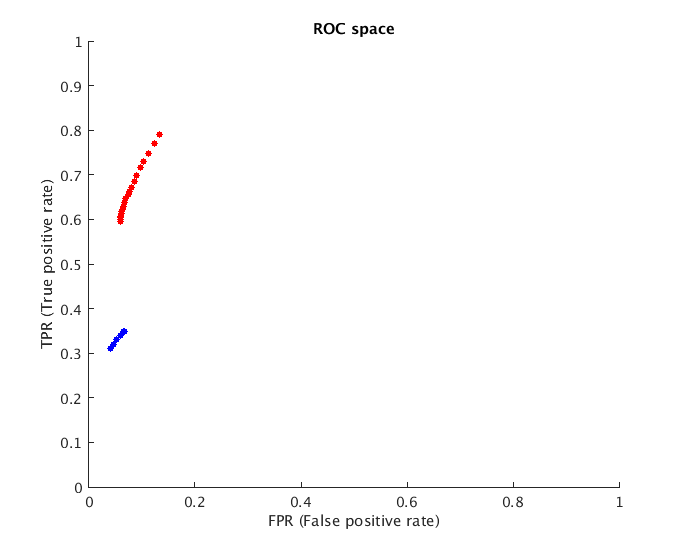
\includegraphics[width=.6\linewidth]{x9343AM/comparison.png}
  \caption{ROC space for CAD (red) and Canny (blue)}
  \label{fig:sub1}
\end{subfigure}
\label{fig:roc_space}
\end{figure}
	
	It can be noted that Canny does not perform very well (sensitivity under 0.4).
	However if we apply anisotropic diffusion,
	sensitivity increases drastically (over 0.8). This happens because the input image
	is very dark at the borders and Canny looses information in the smoothing
	step as well as in the non-maximum suppression step. Supporting this statement
	are the results of applying Canny to 43590 AM (which is very dark compared to
	the other two images and therefore a high smoothing).
	
	A summary of the whole data using the optimal parameters (\textbf{for the FULL evaluation graphs and tables please visit this site:}):
	
\begin{table}[H]
\centering
\caption{Overall results (1: 9343 AM, 2: 10905JL, 3: 43590AM)}
\label{my-label}
\begin{tabular}{|c|c|l|l|}
\hline
\multicolumn{1}{|l|}{Edge detector} & \multicolumn{1}{l|}{Image} & Sensitivity & Specificity \\ \hline
\multirow{3}{*}{Otsu}               & 1                          & 0.9225      & 0.9974      \\ \cline{2-4} 
                                    & 2                          & 0.9279      & 0.9957      \\ \cline{2-4} 
                                    & 3                          & 0.8813      & 0.9958      \\ \hline
\multirow{3}{*}{Sobel}              & 1                          & 0.8498      & 0.8638      \\ \cline{2-4} 
                                    & 2                          & 0.8953      & 0.8852      \\ \cline{2-4} 
                                    & 3                          & 0.8195      & 0.8237      \\ \hline
\multirow{3}{*}{Roberts}            & 1                          & 0.8477      & 0.8400      \\ \cline{2-4} 
                                    & 2                          & 0.8646      & 0.8779      \\ \cline{2-4} 
                                    & 3                          & 0.7540      & 0.8215      \\ \hline
\multirow{3}{*}{Canny}              & 1                          & 0.3404      & 0.9408      \\ \cline{2-4} 
                                    & 2                          & 0.3057      & 0.9863      \\ \cline{2-4} 
                                    & 3                          & 0.2396      & 0.9808      \\ \hline
\multirow{3}{*}{CAD}                & 1                          & 0.7910      & 0.86651     \\ \cline{2-4} 
                                    & 2                          & 0.8139      & 0.9204      \\ \cline{2-4} 
                                    & 3                          & 0.6734      & 0.8921      \\ \hline
\multirow{3}{*}{Dilate-Erode}       & 1                          & 0.8299      & 0.8058      \\ \cline{2-4} 
                                    & 2                          & 0.8003      & 0.8119      \\ \cline{2-4} 
                                    & 3                          & 0.7446      & 0.7863      \\ \hline
\multirow{3}{*}{LoG}                & 1                          & 0.2250      & 0.9419      \\ \cline{2-4} 
                                    & 2                          & 0.2135      & 0.9324      \\ \cline{2-4} 
                                    & 3                          & 0.1996      & 0.9207      \\ \hline
\multirow{3}{*}{DoG}                & 1                          & 0.2137      & 0.9857      \\ \cline{2-4} 
                                    & 2                          & 0.2446      & 0.9941      \\ \cline{2-4} 
                                    & 3                          & 0.17301     & 0.99094     \\ \hline
\end{tabular}
\end{table}
	
	\section{Conclusion}

	From the evaluation Otsu's method performed the best in all input images:
	
\begin{table}[H]
\centering
\caption{Otsu evaluation}
\label{otsu}
\begin{tabular}{@{}llll@{}}
\toprule
Image    & Sensitivity & Specificity & Threshold \\ \midrule
9343 AM  & 0.9225      & 0.9974      & 0.0902    \\
10905 JL & 0.9279      & 0.9957      & 0.1333    \\
43590 AM & 0.8813      & 0.9958      & 0.0510    \\ \bottomrule
\end{tabular}
\end{table}

	It can be noted that Canny does not perform very well (sensitivity under 0.4).
	However if we apply anisotropic diffusion,
	sensitivity increases drastically (over 0.8). This happens because the input image
	is very dark at the borders and Canny looses information in the smoothing
	step as well as in the non-maximum suppression step. Supporting this statement
	are the results of applying Canny to 43590 AM (which is very dark compared to
	the other two images and therefore a high smoothing).

\end{document}